%
% Copyright (C) 2017 Jan Nowotsch
% Author Jan Nowotsch	<jan.nowotsch@gmail.com>
%
% Released under the terms of the GNU GPL v2.0
%



\chapter{Architecture Abstraction\label{chap:arch}}
	The architecture interface implements an abstraction layer for the actual target hardware. It provides the interface between the target hardware and the kernel, cf. Chapter~\ref{chap:kernel}.


\section{Interface Header}
	\begin{description}
	\item[include/arch/arch.h]
		\hyperref[arch_8h]{include/arch/arch.h} is the main architecture header file. It provides access to the architecture implementation defined through \lstinline{CONFIG_ARCH_HEADER}. The header includes the respective architecture header and provides macros to call kernel and common functions as well as a macro to access architecture information. Therefor, it also defines the types containing the architecture interface callback functions, which are \hyperref[structarch__ops__kernel__t]{arch\_ops\_kernel\_t} for kernel and \hyperref[structarch__ops__common__t]{arch\_ops\_common\_t} for common callbacks.

	\item[include/arch/*]
		The remaining header files in \lstinline{include/arch} contain wrapper macros to access all of the architecture interface functions separately.
	\end{description}


\section{Defining an Architecture}
	The following is required to implement support for a target architecture.

	\subsection{Types}
		\begin{itemize}
			\item \lstinline{struct thread_ctx_t}: struct to store the processor context
		\end{itemize}

	\subsection{Callback Functions}
		The callback functions are registers by defining variables of type \hyperref[structarch__ops__kernel__t]{arch\_ops\_kernel\_t} and \hyperref[structarch__ops__common__t]{arch\_ops\_common\_t} named \lstinline{arch_ops_kernel} and \lstinline{arch_ops_common}.

	\subsection{Interrupt Handling and Nesting}
		The architecture layer is responsible for handling interrupts and passing control to the kernel where necessary, e.g. for system calls. For all interrupts that pass control to the kernel, the interrupted thread's context needs to be saved properly and stored to the currently running thread, cf. \hyperref[kernel_2sched_8c_a34a33397e7197f803feffb423ce6717a]{sched\_running()}. That is, such interrupts may be used as preemption points and cause the active thread to switch.

		In general the architecture layer may decide on interrupt nesting. However, in most cases it should be sufficient to let the kernel decide.

		Further, the architecture interrupt implementation is responsible to:
		\begin{enumerate}
			\item preserve the kernel \hyperref[errno_8h_ad65a8842cc674e3ddf69355898c0ecbf]{errno} variable
			\item reset \hyperref[errno_8h_ad65a8842cc674e3ddf69355898c0ecbf]{errno} before passing control to kernel handlers
		\end{enumerate}

	\subsection{System Calls}
		The system call implementation is required to:
		\begin{enumerate}
			\item kernel: update the errno member of \hyperref[sys_2syscall_8h_structsc__arg__t]{sc\_arg\_t}
			\item user space: update \hyperref[errno_8h_ad65a8842cc674e3ddf69355898c0ecbf]{errno}
		\end{enumerate}

	\subsection{Kconfig}
		\begin{itemize}
			\item a respective \quote{Processor type} has to be added
			\item the \it{hidden} CONFIG variables in \lstinline{arch/Kconfig} need to be defined/selected
		\end{itemize}

	\subsection{Build System}
		\begin{itemize}
			\item libbrick.o shall containing all objects that are required to be linked against applications
			\item linker script scripts/linker/kernel\_$<$arch$>$.lds
			\item memory layout print (optional): scripts/memlayout/main.c, if target specific sections are required
				\begin{itemize}
					\item mandatory memory sections shall be printed using \lstinline{PRINT_RANGE_EE}
					\item optional memory sections shall be printed using \lstinline{PRINT_RANGE}
				\end{itemize}

			\item memory layout check: scripts/memlayout/check.c, if target specific sections shall be checked add them to the \lstinline{regs} array.
		\end{itemize}

\vfill
\pagebreak
\section{Atmel \avr}
	This section summarises some critical specifics of the \avr architecture.

	\subsection{Linker sections}
		The \avr memory is split into code (flash) and data (\gls{sram}). Since the \gls{sram} is volatile memory all data that belong to linker sections such as .data and .bss are initially programmed to the flash memory and need to be copied to \gls{sram} during startup. The respective section offsets are defined in the linker scripts used to link the kernel (\fileref{scripts/linker/kernel\_avr.lds}). In case of the .data section, the base address within the flash is defined as \lstinline{__data_load_start} while the end address is defined as \lstinline{__data_load_end}. The respective target address in \gls{sram} are defined in \lstinline{__data_start} and \lstinline{__data_end}.

	\subsection{Interrupt Handling and Reset}
		At reset execution is started at the processor reset address. The location of the reset address is controlled through the \lstinline{BOOTRST} fuse and might be at the start of the application section (\lstinline{0x0}) or the boot loader. The start of the boot loader section is further controlled through the \lstinline{BOOTSZ0, BOOTSZ1} fuse bits. Depending on the memory configuration of the target controller the boot loader start address may vary.
		
		Depending on the fuse bit configuration the kernel base address has to be set through\\\lstinline{CONFIG_KERNEL_TEXT_BASE}. \remark{It shall be noted that the application flash is address is 2-byte chucks, hence addresses listed in the manual need to be multiplied by two in order to get the byte address.}

		The location of the interrupt vectors (except the reset vector) is controlled through \lstinline{MCUCR[IVSEL]}. They can either be placed at the start of the application section or the boot loader section. In the current implementation all interrupt vectors, including the reset vector, are mapped to the same location depending on \lstinline{CONFIG_KERNEL_TEXT_BASE}.

%
% Copyright (C) 2020 Jan Nowotsch
% Author Jan Nowotsch	<jan.nowotsch@gmail.com>
%
% Released under the terms of the GNU GPL v2.0
%



\section{x86emu}
	The x86emu is intended to run \brickos on an x86 host. Figure~\ref{fig:x86emu_components} summarises the main components.

	\begin{figure}[h]
		\centering	
		\includegraphics[scale=.75]{arch/x86emu_components}
		\caption{x86emu components.}
		\label{fig:x86emu_components}
	\end{figure}

	The emulator uses one process each for the kernel, the user space application and the actual emulator itself. The interface between those processes are \gls{ipc} pipelines and signals which emulate hardware events/operations, such as interrupts and hardware state controls.

	The emulator process implements threads with the following responsibilities:
	\begin{description}
		\item[Signal Handler] Processing of hardware requests from the kernel and user space processes. Application state handling, especially shutdown and broken communication to the kernel and user space processes.
		\item[Hardware Event Handler] Process hardware events.
		\item[Interrupt Controller] Trigger hardware requests to the kernel.
		\item[Timer] Periodically enqueue timer interrupts.
		\item[User Input] In interactive mode the emulator is controlled by user inputs, which are handled by this thread.
	\end{description}

	The kernel and user space processes are single-threaded. Hence, the only mechanism to interact with them is through signal handlers. Signal handlers cannot be interrupted themselves, thus the protocol used for hardware operations and the mutex between the hardware event handler and the interrupt controller thread ensure that there is only a single ongoing hardware event.

	\subsection{Hardware Event/Operation Protocol}
		Figure~\ref{fig:x86emu_protocol} depicts the protocol to trigger, process and complete a hardware operation.

		\begin{figure}[h]
			\centering	
			\includegraphics[scale=.75]{arch/x86emu_protocol}
			\caption{Hardware event/operation protocol.}
			\label{fig:x86emu_protocol}
		\end{figure}

		An operation is initiated by the requester sending one of the \gls{ipc} signals to the target. For synchronisation and to acknowledge the request the target sends a sequence number. The requester blocks until the sequence number is available. Once synchronised the actual operation data are exchanged.

		As an additional step for either kernel or application, the acknowledge phase is used to postpone an operation. If an operation is not acknowledged the sender has to restart the operation by waiting for the transmission of the sequence number.

		During processing further data might be exchanged.

		Once processing is complete the operation's write-back phase is again used for synchronisation. The requester blocks while waiting for the results being transfered. The target writes the results. To acknowledge the reception of the results, the requester responds with a sequence number which is read by target.

		Upon completion of the write-back phase both, requester and target, are known to have completed all relevant operations and are clear to trigger or accept a new operations.

